%!TeX root = Thesis_LP.tex
% \sisetup{
% list-final-separator= { and },    % Place "et" à la fin de la liste
% range-phrase= { to }             % Place "à" à entre la gamm
% }

\pagestyle{fancy}
\fancyhf{}
\renewcommand{\headrulewidth}{0pt}
\fancyhead[LO]{\emph{Article 2. Stochastic \ce{CO2} monitoring}}
\fancyhead[RO]{\thepage}
\fancyhead[LE]{\thepage}


\chapter{Stochastic inversion workflow using the gradual deformation to estimate
reservoir properties and predict the \texorpdfstring{\ce{CO2}}{CO2} distribution
within a saline aquifer}
\label{ch:article2}
\selectlanguage{english}

\chaptermark{Stochastic \ce{CO2} monitoring} % Titre court apparaissant dans
% l'entête des pages

{\setlength{\parindent}{0cm}
\underline{\textbf{Titre traduit}}\\
Flux de travail d'inversion stochastique utilisant la déformation graduelle
pour estimer les propriétés de réservoir afin de prédire la distribution du
\ce{CO2} dans un aquifère salin.

\underline{\textbf{Auteurs}}\\
Lorenzo Perozzi$^1$, Erwan Gloaguen$^1$, Bernard Giroux$^1$\\
$^1$ Institut national de la recherche scientifique - Centre Eau Terre
Environnement, 490, de la Couronne, Qu\'ebec, QC, G1K 9A9, CANADA

\newpage
\underline{\textbf{Contribution}}
{\setstretch{1.0}
\begin{description}[leftmargin=!,labelwidth=\widthof{\bfseries Erwan Gloaguen}]
  \setlength\itemsep{0.7em}
  \item[Lorenzo Perozzi] Conceptualisé et réalisé (les mesures de laboratoire,
la modélisation sismique, l’interprétation des résultats) l’étude et rédigé
l’article
  \item[Erwan Gloaguen]  Conceptualisé l'étude, fourni des conseils sur
l’interprétation des résultats et contribué à la rédaction de l’article.
  \item[Bernard Giroux]  Contribué à la rédaction de l’article. \\
\end{description}
}

\underline{\textbf{Publication ciblée}}\\
{\setstretch{0.5}
Computational Geosciences\\
à soumettre\\
}

\underline{\textbf{Résumé traduit}}\\
En raison de contraintes financières, la séquestration géologique du \ce{CO2}
dans les aquifères salins est souvent effectuée en utilisant uniquement un puits
injecteur et un puits de surveillance, ce qui limite sérieusement la
compréhension de la dynamique du panache de \ce{CO2}. Dans ce cas, la
surveillance du \ce{CO2} repose uniquement sur des hypothèses géologiques ou sur
les données indirectes. Dans ce travail, on présente une nouvelle approche en
deux étapes pour l'inversion des ondes $P$ et $S$, de la densité et de la
porosité permettant une prédiction fiable
de la distribution du \ce{CO2}. Dans la première étape, on calcule plusieurs
ensembles de modèles stochastiques des propriétés élastiques en utilisant des
cosimulations séquentielles gaussiennes. Les réalisations de chaque ensemble
sont ensuite combinées entre elles de façon itérative en utilisant une technique
d'optimisation par déformation graduelle où la différence entre les traces
sismiques calculées et observées devient la fonction objectif. Dans la deuxième
étape, les résultats obtenus de l'étape précédente constituent les modèles
d'entrée pour le calage historique, toujours par déformation graduelle, de
l'injection du \ce{CO2}. À chaque itération, on simule l'écoulement du \ce{CO2}
et on calcule les traces sismiques correspondantes qui sont comparées aux traces
observées. Ce flux de travail a été testé sur un modèle hétérogène qui reproduit
l'environnement que l'on retrouve dans la région de Bécancour au Québec. Les
résultats montrent que les modèles optimisés ont une plus grande similarité
structurale avec les modèles de référence, comparée aux simulations
conventionnelles.
}

\section{Abstract}
Due to budget constraints, CCS in deep saline aquifers is often carried out
using only one injector well and one control well, which seriously limits
the understanding of the \ce{CO2} plume dynamics. In such case, monitoring of the
plume of \ce{CO2} only relies on geological assumptions or indirect data. In this
paper, we present a new two-step stochastic $P$- and $S$-waves, density and
porosity inversion approach that allows reliable monitoring of \ce{CO2} plume
using time-lapse VSPs. In the first step, we compute several sets of stochastic
models of the elastic properties using conventional sequential Gaussian
cosimulations. Each realization within a set of static models are then
iteratively combined together using a modified gradual deformation optimization
technique with the difference between computed and observed raw traces as
objective function. In the second step, these statics models serve as input for
a \ce{CO2} injection history matching using the same modified gradual
deformation scheme. At each gradual deformation step the \ce{CO2} injection is
simulated and the corresponding full-wave traces are computed and compared with
the observed data. The method has been tested on a synthetic heterogeneous
saline aquifer model mimicking the geological environment of the
Becancour area, Quebec. The results show that the set of optimized models of
$P$- and $S$-waves, density and porosity showed an improved structural similarity
with the reference models compared to conventional simulations.
\section{Introduction}
One of the major challenges limiting large-scale deployment of Carbon Capture
and Storage (CCS) operations is the issue of evaluating and forecasting the fate
of \ce{CO2} in deep rock formations. The characteristics of the reservoir
determined from the very beginning the design and operational conditions of most
of the CCS chain.  Indeed, having a comprehensive knowledge of the physical
characteristics of the storage site is crucial to determine the optimal rate of
\ce{CO2} injection, which influences the rate of capture, as well as the
parameters of a proper monitoring strategy.  Let us recall that monitoring is an
essential component of any CCS project and that most, if not all, jurisdictions
require more or less elaborated monitoring, verification and accounting (MVA)
programs (e.g.\ European CCS directive \citep{EU2014}).\\
A common task in CCS projects is thus to monitor the spatial distribution of
\ce{CO2} over time. However, the spatial distribution of the \ce{CO2} plume that
is estimated through monitoring is often inconsistent, to varying degrees, with
model-based simulations \citep{Ramirez2013}. This is mainly due to the lack or
sparseness of direct measurements of the reservoir petrophysical properties,
the low spatial coverage of geophysical surveys,  the underlying resolution of
inversion techniques and to uncertainties that limits the understanding of the
subsurface and therefore the ability to produce accurate reservoir models
allowing reliable forecasts of the \ce{CO2} plume.\\
The process of optimizing a reservoir model to fit dynamic data is commonly
known as history matching and is extensively used in the oil and gas industry \citep{Roggero1998}.
In conventional history matching, the target variables are reservoir engineering
properties such as pressure, water-cut, rate of production of oil, and the like,
all involving at least one injector and one pumping well. In \ce{CO2} storage
projects, such well configuration is not conceivable (pumping is not done) and
only one injector well is usually available. In this context, only indirect data
have the spatial coverage and the potential to improve the estimation of the
\ce{CO2} plume within the deep saline aquifers.\\
History matching requires the knowledge, at least in the stochastic sense, of
the spatial distribution of the static properties of the reservoir (porosity,
permeability). Due to the geological complexity and the scarcity of direct
observations (i.e.\ well data), probabilistic methods appear to be the most
suitable choice to build a reliable reservoir model. In addition, it is
established that seismic measurements are well suited to constrain static
reservoir properties modeling as they provide indirect but correlated and
spatially extensive information about reservoir properties \citep{Doyen2007}.\
The estimation of static parameters from seismic data is a complex,
ill-conditioned, nonlinear inverse problem due principally to the limited
bandwidth  of the seismic data, noise, measurement errors,
and  the assumptions underlying to forward models \citep{Tarantola2004}.
Seismic inverse problems may be developed following deterministic or
probabilistic approaches and can be divided into two main categories: (1)
multiple step inversion methods and (2) stochastic inversion methods
\citep{Grana2012}.\\
In multiple step inversion methods, the problem of estimating reservoir
properties from seismic data is split into two or more subproblems; elastic
properties are first derived from partial stacked seismic data through elastic
inversion; then, reservoir properties are classified by statistical techniques,
such as Bayesian classification \citep{Avseth2001,Mukerji2001,Buland2003}.\\
Iterative stochastic inversion methodologies solve the seismic inverse problem
using deterministic or stochastic optimization techniques. First, a set of
equivalent earth models is simulated using a stochastic algorithm based on prior
information usually from available well log data and a spatial continuity
pattern (e.g.\ variogram, training image) to create fine-scale reservoir models
\citep{Bosch2009}. Then suitable rock-physics transforms are applied to generate
the corresponding volumes of the elastic properties. Finally, synthetic seismic
volumes are computed and compared to real seismic data to evaluate the mismatch.
Several optimization methods exist to infer the elastic properties based on the
measured traces. \citet{Gonzalez2008} performed a trace-by-trace deterministic
optimization, \citet{Bosch2009} proposed an iterative optimization based on
Newton's method; Markov chain Monte Carlo approach has been used successfully
for the stochastic exploration of the model space
\citep{Eidsvik2004,Larsen2006,Gunning2007,Rimstad2010,Ulvmoen2010,Hansen2012}.
\citet{Grana2012} show the efficiency of the probability perturbation method
\citep{Caers2006} to estimate fine-scale reservoir models in a stochastic
inversion. A multidimensional scaling technique was successfully applied by
\citet{Azevedo2013} to asses how the parameter model space is explored by global
elastic inversion algorithm.
In addition to the static information and in order to evaluate the performance
of the reservoir in terms of \ce{CO2} storage, reservoirs models need to be
constrained by dynamic data obtained from the \ce{CO2} injection operations. To
be meaningful, reservoir models must match the observed dynamic behavior of the
reservoir within some interval of tolerance. History matching is also an
ill-posed problem and can be solved using the same algorithms as the one used
for estimating the static properties, but then involving the injection data and
forward fluid flow modeling.
In this paper we propose a stochastic inversion workflow using a modified
gradual deformation parametrization method \citep{Roggero1998} as a stochastic
optimization technique that integrates geophysical and geological logs, seismic
reflection data and \ce{CO2} flow simulations in order to analyze and monitor
the \ce{CO2} injection and its propagation within a saline aquifer.  This paper
is organized as follows. In the first section, we focus on each step of the
seismic inversion algorithm. The second section presents an the application of
the approach to characterize a synthetic reservoir for the \ce{CO2} injection in
the St.\ Lawrence Lowlands, Quebec, Canada.
\section{Methodology}
\label{sc:metho_art2}
The flowchart of the stochastic inversion that we propose is shown in
\cref{fig:workflow}.  It is a three step approach. Firstly, many sets of initial
realizations are simulated from available static data (well logs, deterministic
elastic inversion, etc.) using a geostatistical cosimulation algorithm.
Secondly, an optimization loop is applied to each set before modeling \ce{CO2}
injection in order to obtain a static model of petrophysical properties that
maximize the match between computed and observed seismic traces. Finally, the
resulting models are then combined in an iterative history-matching loop where,
at each step, we simulate \ce{CO2} injection and transport, compute the elastic
properties of the corresponding model, and run a seismic forward model to
calculate the mismatch between simulated and observed traces. In the following
sections, we focus on each step of the algorithm.
\begin{figure}[!ht]
\centering
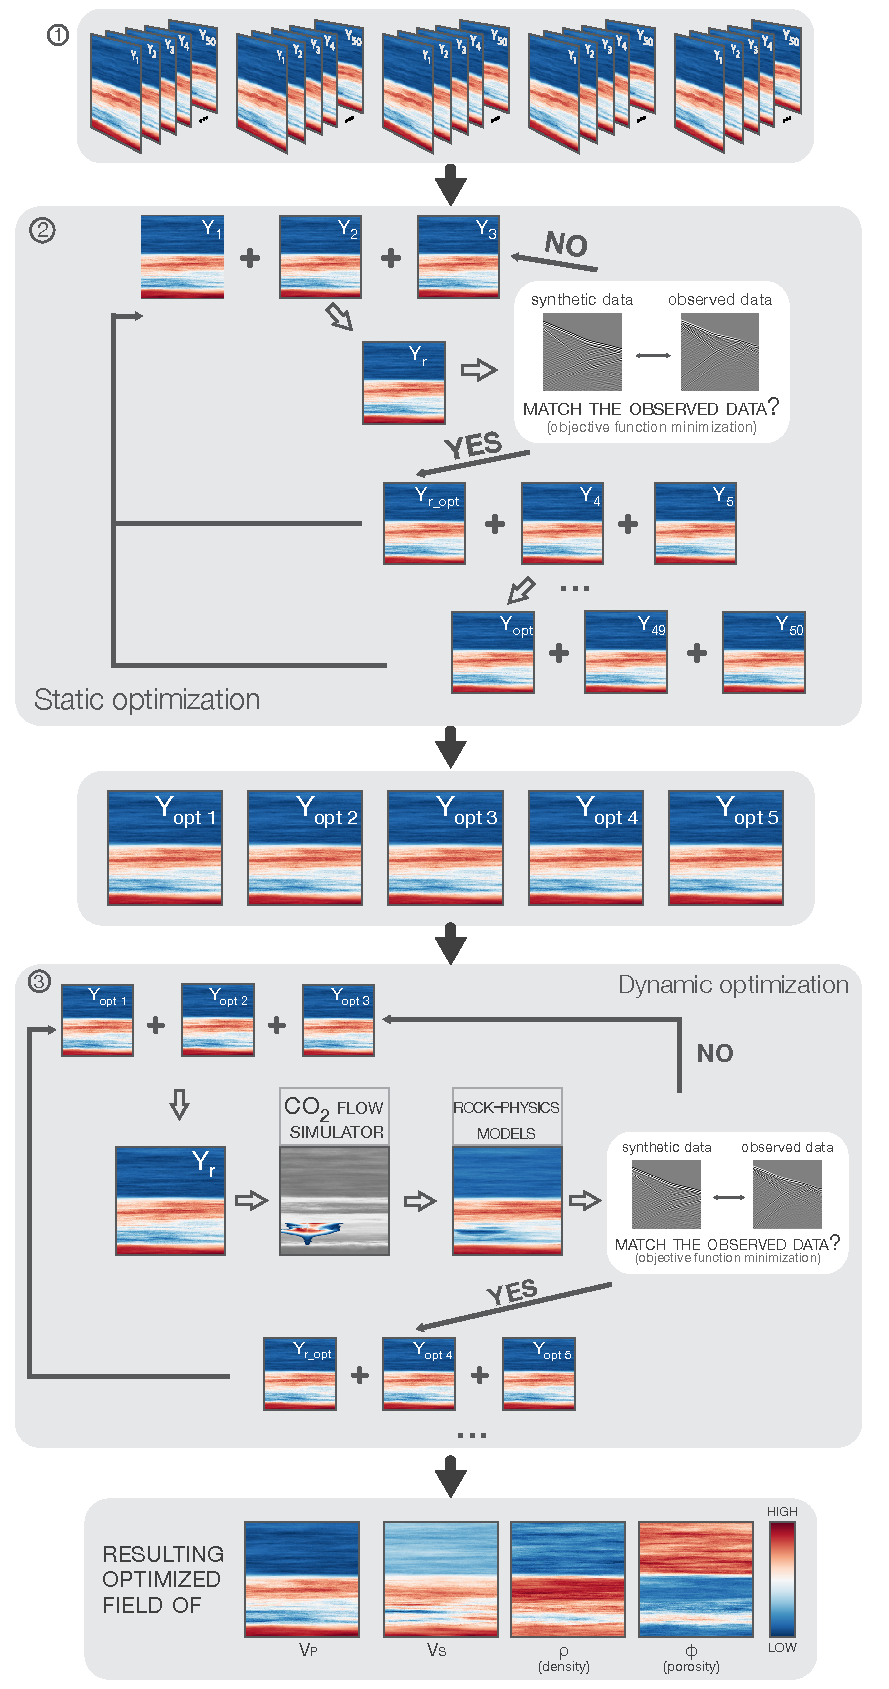
\includegraphics[width=0.68\textwidth]{fig/workflow_authorea.pdf}
\caption{Workflow of the stochastic inversion methodology}
\label{fig:workflow}
\end{figure}
\subsection{Geostatistical methods}
In our approach, $P$ and $S$-wave velocity ($V_p$ and $V_s$), porosity ($\phi$)
and density ($\rho$) are first simulated using Sequential Gaussian CoSimulation
(SGCS) \citep{Deutsch1998,Doyen2007}. SGCS is a method that allows simulating
continuous random variables and that requires only the knowledge of their
variogram, histogram and coefficient of correlation. Starting from prior
information available form well log data, the algorithm visits each node of the
grid along a random path. At each step along this path, the algorithm
co-simulates a series of values for each variable. At each node, the prior
information and the previously simulated values are used to compute the kriging
mean and variance of each variable. This feedback loop ensures that the
simulation is spatially correlated. By construction, SGCS  will be conditioned
to the well data, i.e.\ the simulations reproduce the well observations and thus
have the same overall statistical properties. Multiple simulation are generated
by using different random paths and random seeds in order to obtain independent
sets of realizations. For an extended review about SGCS methods, refer to
\citet{Deutsch1998} and \citet{Doyen2007}.
\subsection{Static optimization}
In the second step of the algorithm, realizations of each set are iteratively
combined using the gradual deformation (GD) method \citep{Hu2000} as a
optimization technique. The GD is a parametrization method that allow to
iteratively perturb a set of realizations until obtaining a new realization that
minimizes the mismatch with some observed data. This method was first developed
for history matching purposes \citep{Roggero1998} and involves the linear
combination of Gaussian random fields with weights that are adjusted to minimize
the data mismatch while preserving the spatial covariance. Many variations of
this technique have since been presented
\citep{Roggero1998,Hu2000,Hu2002,Hu2001,LeRavalec2000,LeRavalec2012}. The key
idea behind the GD is that the sum of two Gaussian random field ($Y1$ and $Y2$)
is also a Gaussian random field:
\begin{equation}
Y(r) = Y_1\ cos(r) + Y_2\ sin(r)
\end{equation}
where $r$ are the gradual deformation coefficient. It can be shown that $Y(r)$
is a realization with the same mean and covariance as $Y_1$ and $Y_2$ whatever
the value of the deformation parameter $r$. This primary gradual combination
scheme involves independent realizations only, meaning that the $Y_1$ and $Y_2$
realizations are unconditional. To combine conditional realization, a variant of
the GD named gradual conditioning (GC) method was developed by \citet{Ying2000}
and \citet{Hu2002}. In this case, the  weights have to satisfy a new constraint.
Their sum has to be one while their sum to the square is also one. Within this
conditions, the realization built from two conditional realizations is also
conditional to the measured data and reproduce the overall covariance.
\citet{Hu2002} proposes the weights parametrization as follows:
\begin{equation}
\begin{cases}
    \alpha_1 = \dfrac{1}{3} + \dfrac{2}{3}\ cos(r)\\
    \alpha_2 = \dfrac{1}{3} + \dfrac{2}{3}\ sin\bigg(-\dfrac{\pi}{6}+r\bigg)\\
    \alpha_3 = \dfrac{1}{3} + \dfrac{2}{3}\ sin\bigg(-\dfrac{\pi}{6}-r\bigg)
    \end{cases}
\end{equation}
with parameter $r \in [-\pi,\pi]$. In comparison with the combination of
independent realizations, the above procedure avoids the conditioning step
during the optimization process.\\

When the GC method is incorporated into the optimization processes, the
deformation parameter $r$ becomes the parameter to adjust to reduce the
objective function.  At this stage, for each combination (i.e.\ for each value
of $r$) we obtain a new $V_p$, $V_s$ $\rho$ and $\phi$ field model. Afterwards,
the full-wave synthetic seismic response of the earth models $d_{synth}$ is
computed using an elastic finite-difference time-domain approach
\citep{Bohlen2002} and compared to the observed data $d_{obs}$. For this study,
the objective function is defined as the root mean square error between
$d_{obs}$ and $d_{synth}$:
\begin{equation}
J(r) = \sqrt{\frac{1}{N}\sum\limits_{i=1,N}\big(d_{synth}(r)-d_{obs}\big)^2}
\end{equation}
where $N$ is the number of the samples per trace and $i$ the sample index.
The combination for which $r$ minimize the mismatch between synthetic and
observed data is retained and combined with two initial SGCS realizations.
Ultimately, we obtain $V_p$, $V_s$, $\rho$ and $\phi$ fields that have the best
seismic match with the observed data.
\subsection{Dynamic optimization}
The results obtained after the previous step honor the static well-log data and
the variograms inferred from these data and the deterministic static inversion.
The aim now is to make the reservoir model consistent with the dynamic data
(i.e.\ \ce{CO2} injection and propagation within the reservoir). An iterative
history matching loop is started in which each iteration consists of the
following steps:
\begin{enumerate}
	\item run a fluid flow simulation;
	\item apply suitable rock-physics mapping to generate the corresponding volumes
of the elastic properties after \ce{CO2} injection;
	\item compute the seismic response;
	\item calculate the mismatch between simulated and observed data;
	\item perturb the model to lower the mismatch using gradual deformation.
\end{enumerate}
\subsubsection{Flow simulation}
In recent years, vertical-equilibrium (VE) models have been extensively used to
study gravity-driven \ce{CO2} migration \citep{Nordbotten2011}. Using an
analytical description for the vertical fluid distribution not only reduces the
dimensions of the problem but also lessens the coupling and increases the time
constants of the dynamic model \citep{Nilsen2014}. VE models are attractive
means to increase resolution while reducing computational burden, and are thus
particularly attractive for an iterative history-match loop where many flow
simulation steps are required. For the purpose of this study, we used the VE
solvers included in the Matlab Reservoir Simulation Toolbox (MRST)
\citep{Lie2012}, to model injection of CO$_2$ in the saline aquifer.
\subsubsection{Elastic properties}
\label{sc:elasticproperties}
Elastic properties are usually computed through a rock-physics model. This model
is a set of equations that transform petrophysical variables, typically
porosity, mineralogy and fluid saturations, into elastic properties such as $P$-
and $S$-wave velocity and density. For the purpose of this work, we first
estimate the elastic properties of the solid phase, i.e.\ bulk ($K_s$) and shear
($G_s$) moduli, by applying the arithmetic average of the upper and lower
Hashin-Shtrikman bounds \citep{Hashin1963}. Then we compute the elastic
properties of the fluid phase, i.e.\ bulk ($K_f$) modulus and density
($\rho_f$), using fluid mixing laws \citep{Wood1955,Brie1995}. \\
The new \ce{CO2} saturated rock properties $K_{sat}$ is then calculated using
Gassmann's relation \cite{Gassmann}:
\begin{equation}
K_{sat} = K_{dry} + \dfrac{\bigg(1-\frac{K_{dry}}{K_s}\bigg)^2}{\frac{\phi}{K_{fl}}+\dfrac{(1-\phi)}{K_s}-\frac{K_{dry}}{K^2_s}},
\label{eq:gassmann}
\end{equation}
where $\phi$ refers to porosity. The shear modulus of the saturated rock is
simply the modulus of the dry rock ($G_{sat}$=$G_{dry}$).
The saturated density $\rho_{sat}$ is computed as a linear combination of the
solid density $\rho_s$ and fluid density $\rho_{fl}$ weighted by their
respective volume fractions:
\begin{equation}
\rho_{sat} = \phi\ \rho_{fl} + (1 - \phi)\rho_s,
\label{eq:rho2}
\end{equation}
and the new $P$- and $S$-wave velocity are calculated using the saturated
elastic properties $K_{sat}$ and $G_{sat}$ and density $\rho$:
\begin{equation}
\label{eq:Vp2}
V_p = \sqrt{\Bigg(\dfrac{K_{sat}+\tfrac{4}{3}G_{sat}}{\rho_{sat}}\Bigg)},
\end{equation}
and
\begin{equation}
\label{eq:Vs2}
V_s = \sqrt{\dfrac{G_{sat}}{\rho_{sat}}}.
\end{equation}
Then, a synthetic full-wave seismic response $d_{synth}$ is computed  using an
elastic finite-difference time-domain approach \cite{Bohlen2002}.
The mismatch between $d_{synth}$ and $d_{obs}$ is evaluated using the same
objective function of the previous step.
At the end of the stochastic inversion process, we obtain the fields of $V_p$,
$V_s$, density ($\rho$) and porosity ($\phi$) that best honor static and dynamic
data.
\section{Application to a synthetic example}
In the following, we apply the workflow approach to a synthetic model that
represent a potential CCS pilot site in the province of Quebec, Canada.
The Cambrian-Ordovician sedimentary basin of the St.\ Lawrence Platform in
southern Quebec (\cref{fig:map}) has been identified as the most prospective
basin for \ce{CO2} storage in the province \citep{Malo2012}.
\begin{figure}[!ht]
\centering
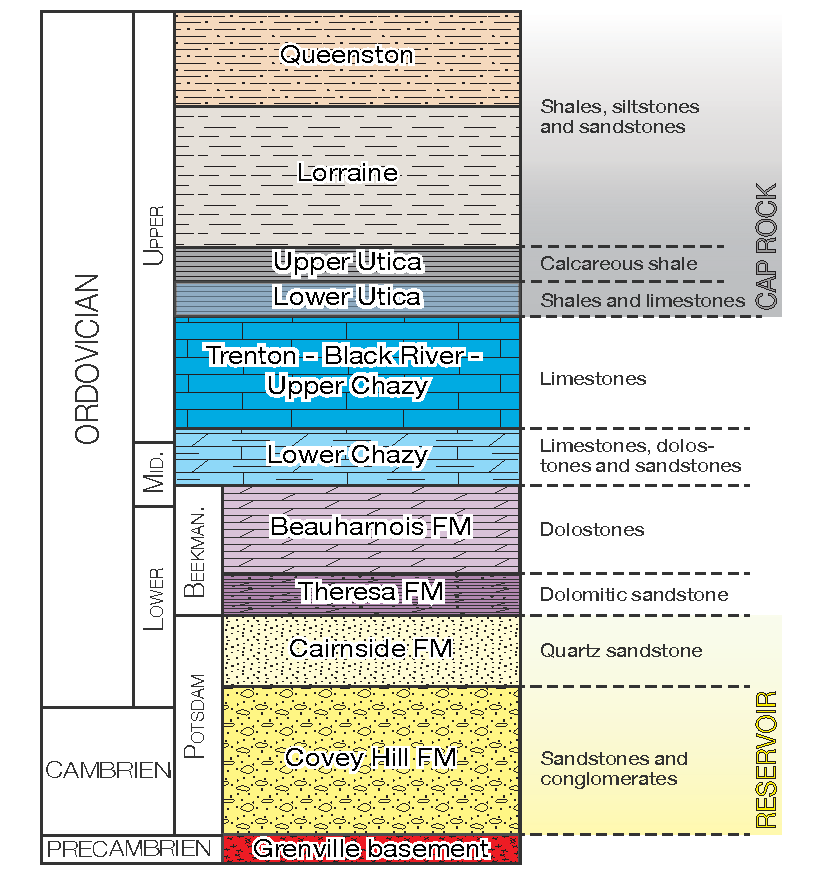
\includegraphics[width=0.8\textwidth]{fig/strati.pdf}
\caption{Simplified stratigraphy of the St. Lawrence Platform. Reservoirs
formations are highlighted in yellow and cap rock formations in light gray.
Modified from \citep{Claprood2012}.}
\label{fig:strati2}.
\end{figure}
The Potsdam Group lies unconformably upon the metamorphic Precambrian Grenville
basement. It is comprised of the Covey Hill (Cambrian sandstones and
conglomerates) and the Cairnside (lower Ordovician quartz sandstone) formations.
The remainder of the section is all of Ordovician age. The Beekmantown Group
includes the Theresa (dolomitic sandstones) and the Beau\-har\-nois (dolostones)
formations. The lower Chazy unit is composed of limestones, dolostones, and
sandstones. The Trenton, Black River, and upper Chazy groups, are limestones.
The Trenton Group is overlain by the Utica Shale and several hundred meters of
interbedded shales, siltstones and sandstones of the Lorraine Group. The lower
Utica Shale comprises limestone beds and is more calcareous than the upper Utica
Shale. Deep saline aquifers are found in the Trenton, Beekmantown and Potsdam
Groups. \Cref{fig:well-log} show synthetic well logs of $V_p$, $\rho$ and $\phi$
representing the complete sedimentary sequence of the St.\ Lawrence Platform,
compiled from a number of log data available in the studied area. $S$-wave
velocity are computed using the Greenberg-Castagna relation
\citep{Greenberg1992}.
\begin{figure}[!ht]
\centering
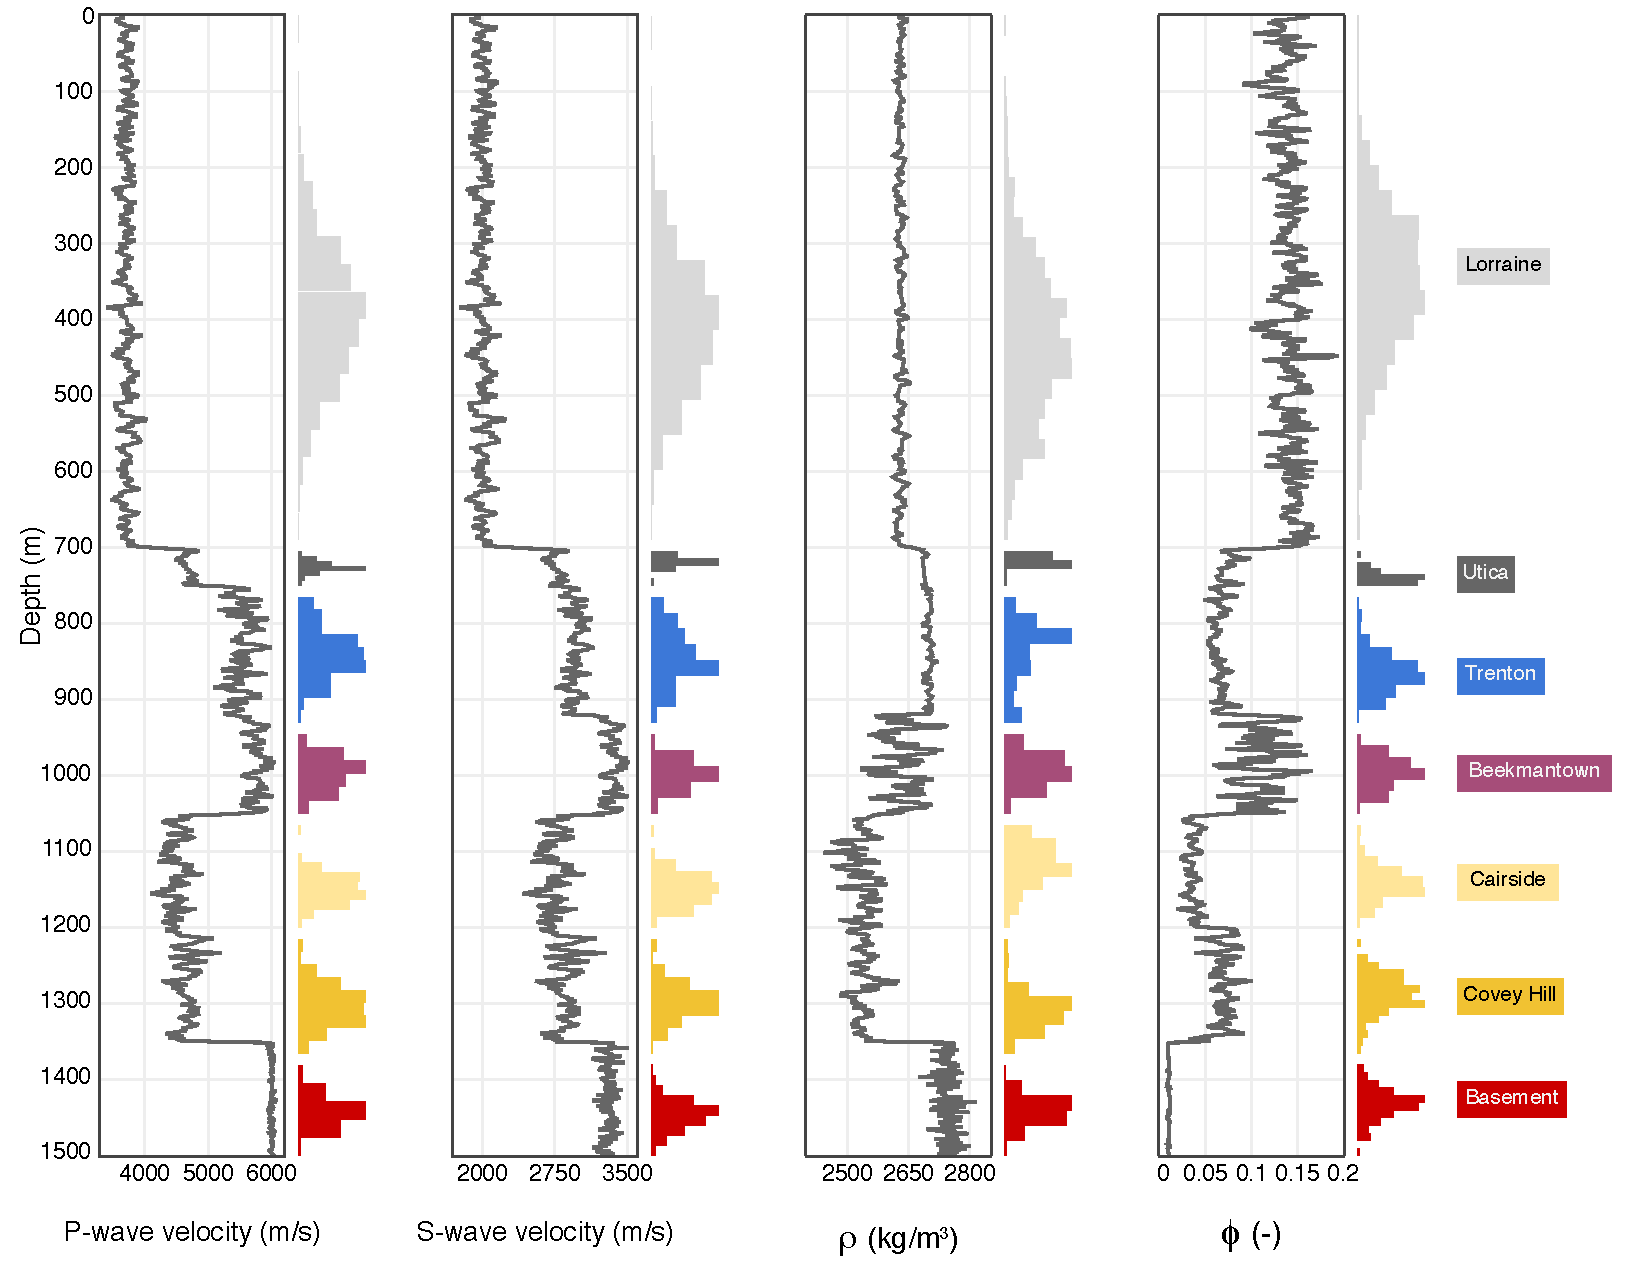
\includegraphics[width=1\textwidth]{fig/well-log.pdf}
\caption{Synthetic well log data set representing the sedimentary sequence of
the St.\ Lawrence Platform. From left to right: $P$-wave and $S$-wave velocity,
density ($\rho$) and effective porosity ($\phi$). For each formation the
corresponding parameter distribution is showed.}
\label{fig:well-log}.
\end{figure}
The sedimentary sequence has been divided in seven groups: Lorraine, Utica
shale, Trenton, Beekmantown, Cairnside, Covey Hill and Basement. For each group,
the well-log parameter distributions are represented in \cref{fig:well-log} and
the mean and standard deviation are summarized on \cref{tab:well-log}.
\begin{table}
\caption{Well-log mean and standard deviation for each group.}
\label{tab:well-log}
\sisetup{
separate-uncertainty,
% table-format = 4.3(1),
}
\centering
\begin{tabular}{
l
SSSS[table-format = 1.2(1)]
}
	\toprule
 		\multicolumn{1}{l}{} &
 		\multicolumn{4}{c}{Well-log parameters}\\
 		\cmidrule(r){2-5}
 		\multicolumn{1}{l}{Group} & \multicolumn{1}{c}{$V_p$} &
\multicolumn{1}{c}{$V_s$} & \multicolumn{1}{c}{$\rho$} &
\multicolumn{1}{c}{$\phi$}\\
 		\multicolumn{1}{c}{} & \multicolumn{1}{c}{(\si{m/s})} &
\multicolumn{1}{c}{(\si{m/s})} & \multicolumn{1}{c}{(\si{kg/m^3})} &
\multicolumn{1}{c}{(-)}\\
	\midrule
	Lorraine   & 3714(98) & 2003(75) & 2629(7) & 0.14(1) \\
	Utica      & 4671(21) & 2750(8) & 2688(5) & 0.07(1)  \\
	Trenton    & 5538(191) & 2958(83) & 2700(10) & 0.06(1)  \\
	Beekmantown& 5766(147) & 3348(85) & 2635(49) & 0.11(2)  \\
	Cairnside  & 4503(172) & 2739(135) & 2537(49) & 0.11(1)  \\
	Covey Hill & 4664(171) & 2849(130) & 2539(26) & 0.07(1)  \\
	Basement   & 6002(30) & 3302(72) & 2746(24) & 0.01(1)  \\
\bottomrule
\end{tabular}
\end{table}
Starting from these distributions, an SGS co-simulation algorithm is used to
generate the reference model of $V_p$, $V_s$, $\rho$ and $\phi$ that are shown
in \cref{fig:ref_model}. The model size is \SI{1000 x 1500}{\metre} with a cell
size of \SI{1 x 1}{\metre}. The simulation algorithm is formulated in order to
respect the natural transition between each group layer.
\begin{figure}[!ht]
\centering
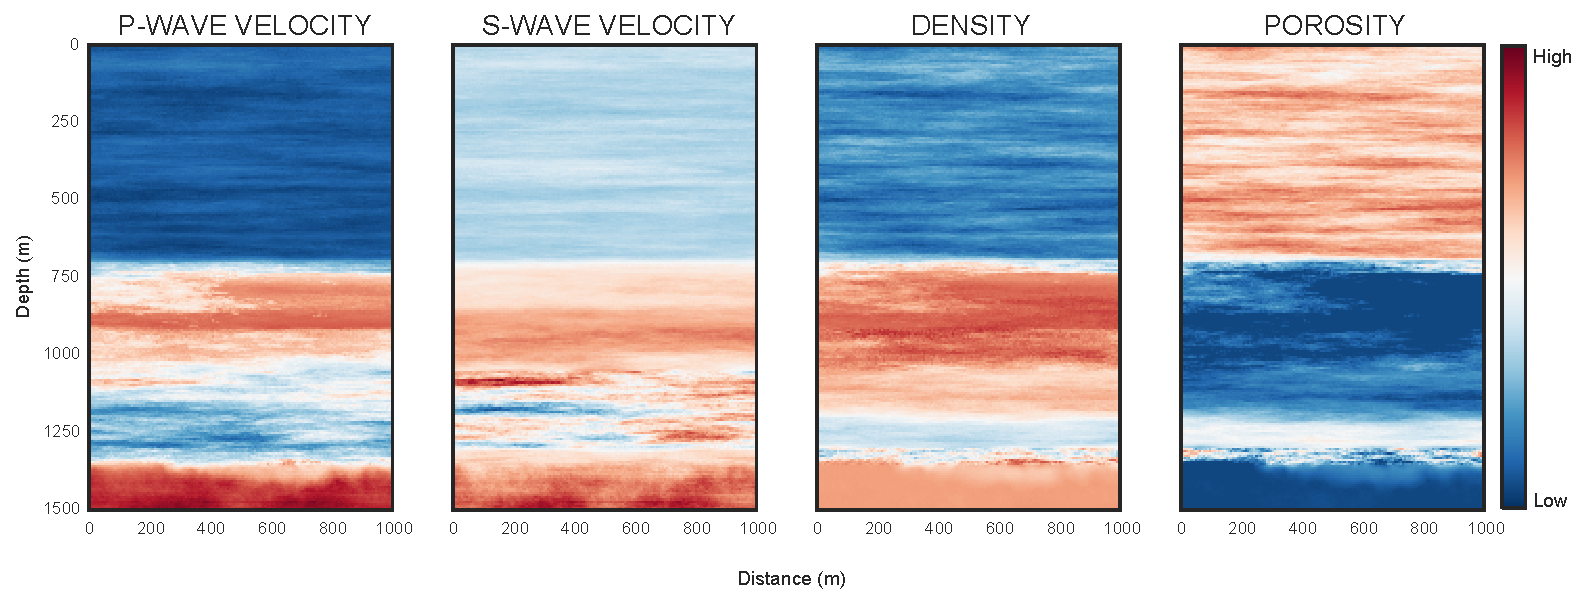
\includegraphics[width=1\textwidth]{fig/ref_model.pdf}
\caption{Reference model for $V_p$, $V_s$, $\rho$ and $\phi$.}
\label{fig:ref_model}.
\end{figure}
The procedure followed in this study to perform seismic modeling on the
reference model is directly inspired by the work of \citet{Carcione2006} who
present an application of poro-viscoelastic modeling for monitoring underground
\ce{CO2} storage. The poro-viscoelastic formulation represents perhaps the most
effective tool to study the effect of the saturating fluid on the seismic
response because fluid properties are directly taken into account in the
equations. A vertical full-wave seismic profile (VSP) for near, mid and large
offset (i.e.\ VSP$_{observed}$) is modeled using the code described in
\citet{Giroux2012}. As the ultimate aim of the inversion workflow is to obtain
an elastic model to predict the \ce{CO2} distribution over time, modeling near,
mid and far offset allow us to take into account every amplitude variation
versus offset due to the fluid substitutions.\\
Starting from three hypothetical well-log of the reference model, we co-simulate
five sets of 100 realizations, each using the SGS algorithm. These realizations
are then linearly combined using the gradual deformation parametrization. At
each parametrization step, a full-wave VSP for near, mid and large offset (i.e,
VSP$_{synth}$) is computed using an elastic finite-difference time-domain
approach \citep{Bohlen2002} and compared to VSP$_{observed}$. At the end of this
iterative process, we obtain the best seismic matched realization for $V_p$,
$V_s$, $\rho$ and $\phi$.\\
The five best seismic matched realizations are then combined again in a gradual
deformation parametrization where at each step we run a \ce{CO2} flow simulator.
The permeability is derived using an extension of the Kozeny-Carman equation
\citep{Kozeny1927,Carman1938} for a packing of identical spheres of diameter $d$
\citep{Mavko2009}:
\begin{equation}
k = \dfrac{1}{72}\dfrac{\phi^3}{(1-\phi)^2\tau^2}d^2,
\end{equation}
where $k$ is the permeability, $\phi$ the porosity and $\tau$ the tortuosity.
The \ce{CO2} is injected during \num{200} days in the Covey Hill formation that
is a low porosity sandstone with a mean spheres diameter of \SI{5e-6}{\metre}.
At each step, the new \ce{CO2} saturated elastic properties of the model are
calculated using \cref{eq:rho2,eq:Vp2,eq:Vs2}, the VSP$_{synth_{200d}}$) is
computed and the mismatch against VSP$_{observed_{200d}}$ is evaluated.\\
The final inversion workflow results for $V_p$, $V_s$, $\rho$ and $\phi$ that
best honor the static data (i.e.\ well-log) and the \ce{CO2} flow within the
reservoir, are shown in \cref{fig:final_model}. These inversion results are then
used to predict \ce{CO2} distributions over time that are validated by the
monitoring data.
\begin{figure}[!ht]
\centering
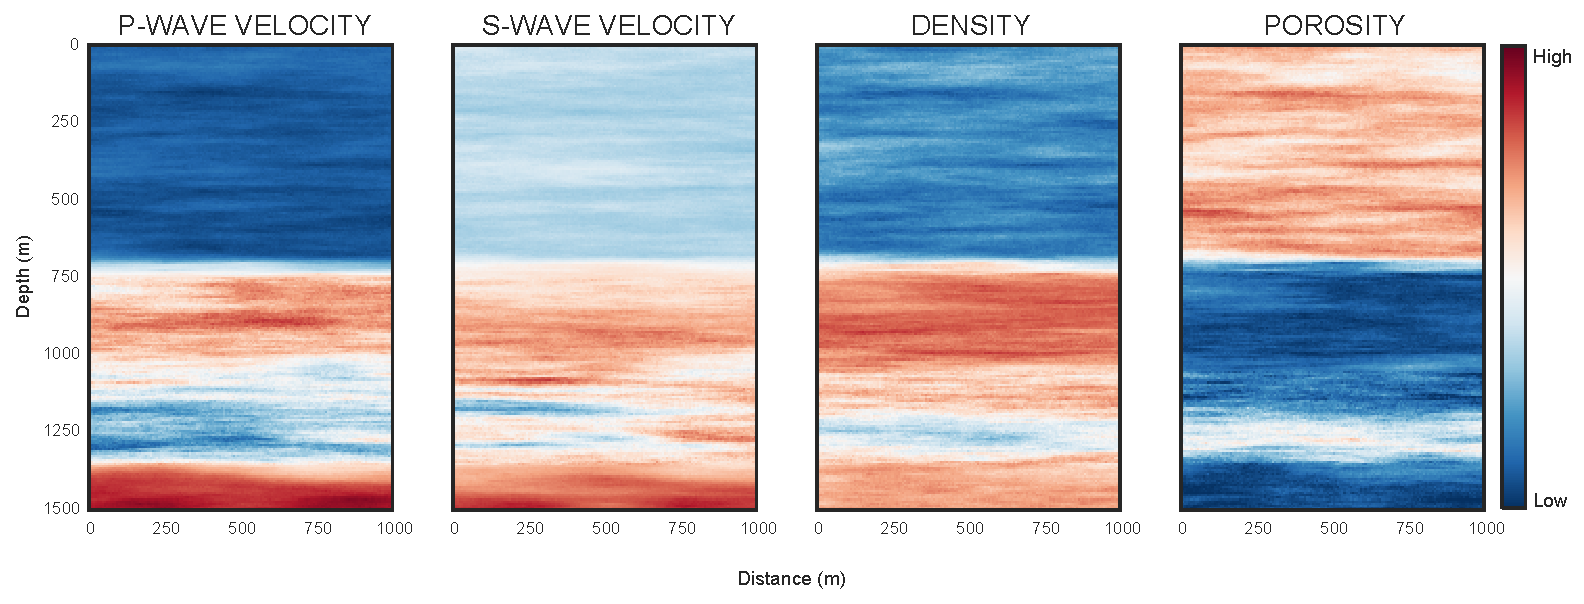
\includegraphics[width=1\textwidth]{fig/final_model.pdf}
\caption{Inversion results for $V_p$, $V_s$, $\rho$ and $\phi$.}
\label{fig:final_model}.
\end{figure}
\subsection{Model Validation}
A statistical analysis is needed to validate the results of our stochastic
inversion approach. \Cref{fig:correlation} shows the correlation between
observed data and one initial SGS realization chosen at random among the set of
100, as well as the correlation between observed data and the final inversion
result. The correlation between observed data and final inversion result is
slightly improved, though the initial set of SGS realizations are already well
correlated with the observed data.
\begin{figure}[!ht]
        \centering
        \begin{subfigure}[b]{1\textwidth}
        		\caption{}
                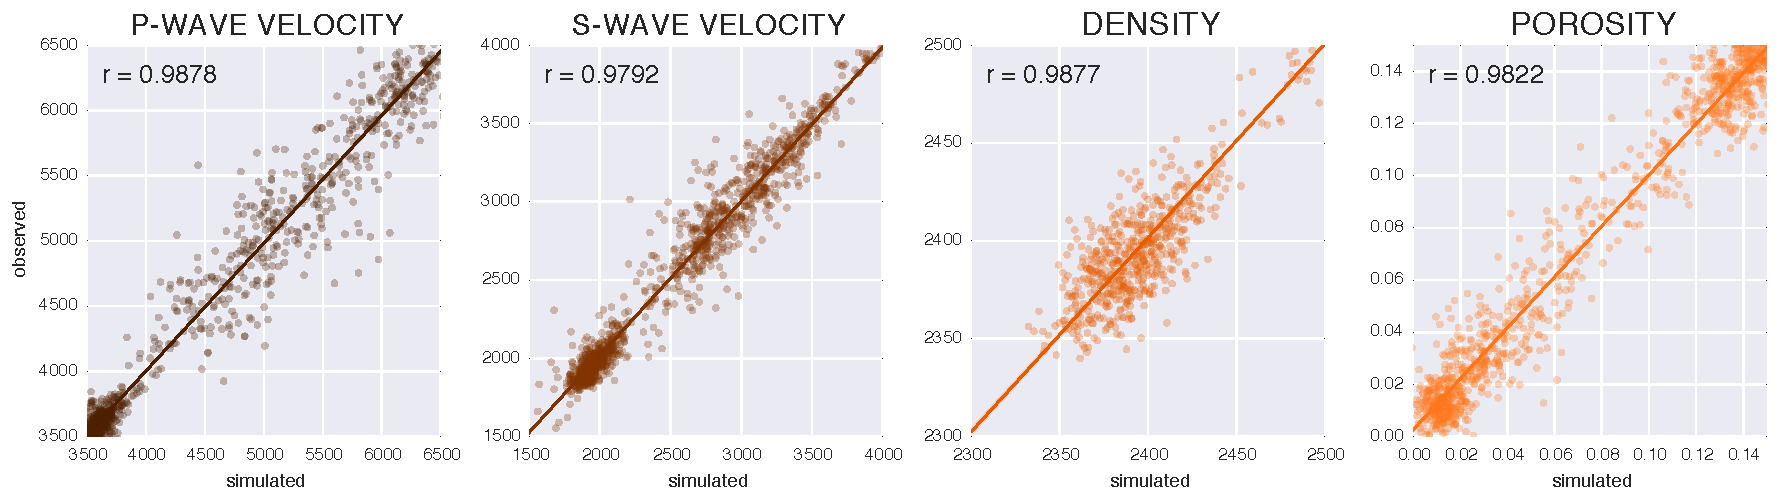
\includegraphics[width=\textwidth]{fig/correlation_a.pdf}
                \label{fig:correlation_a}
        \end{subfigure}%

        \begin{subfigure}[b]{1\textwidth}
                \caption{}
                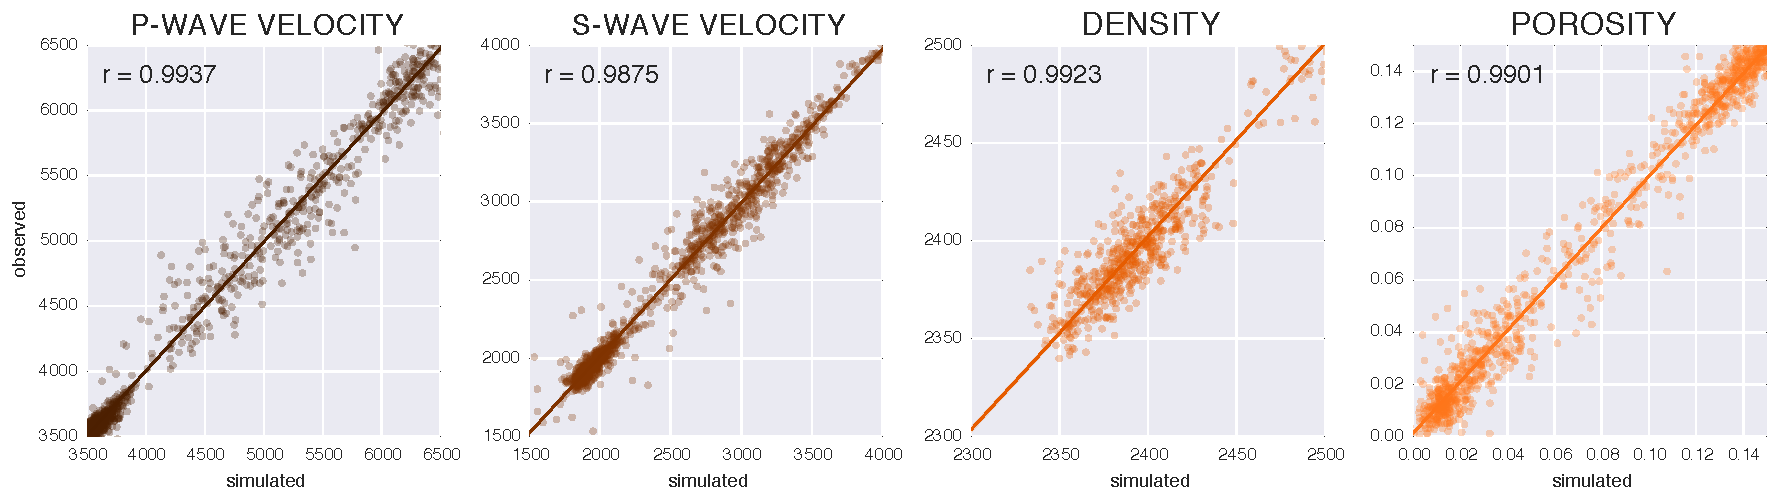
\includegraphics[width=\textwidth]{fig/correlation_b.pdf}
                \label{fig:correlation_b}
        \end{subfigure}
		\caption{Correlation plot for $V_p$, $V_s$, $\rho$ and $\phi$ between observed
data and one initial SGS realization chosen at random among 100 (a) and between
observed data and the final inversion result (b).}
		\label{fig:correlation}
\end{figure}
It is also important to obtain a result that honor the original distribution
(i.e.\ the observed data). The quantile-quantile (q-q) plot is best suited to
study how much two different distributions are similar. \Cref{fig:qqplot} shows
the q-q plot for the reference model and the inversion result for $V_p$, $V_s$,
$\rho$ and $\phi$. A \num{45}-reference line is also plotted in red. Since
almost all the points fall along the reference line, we consider that the
inversion results distributions are the same as the observed distributions.
\begin{figure}[!ht]
\centering
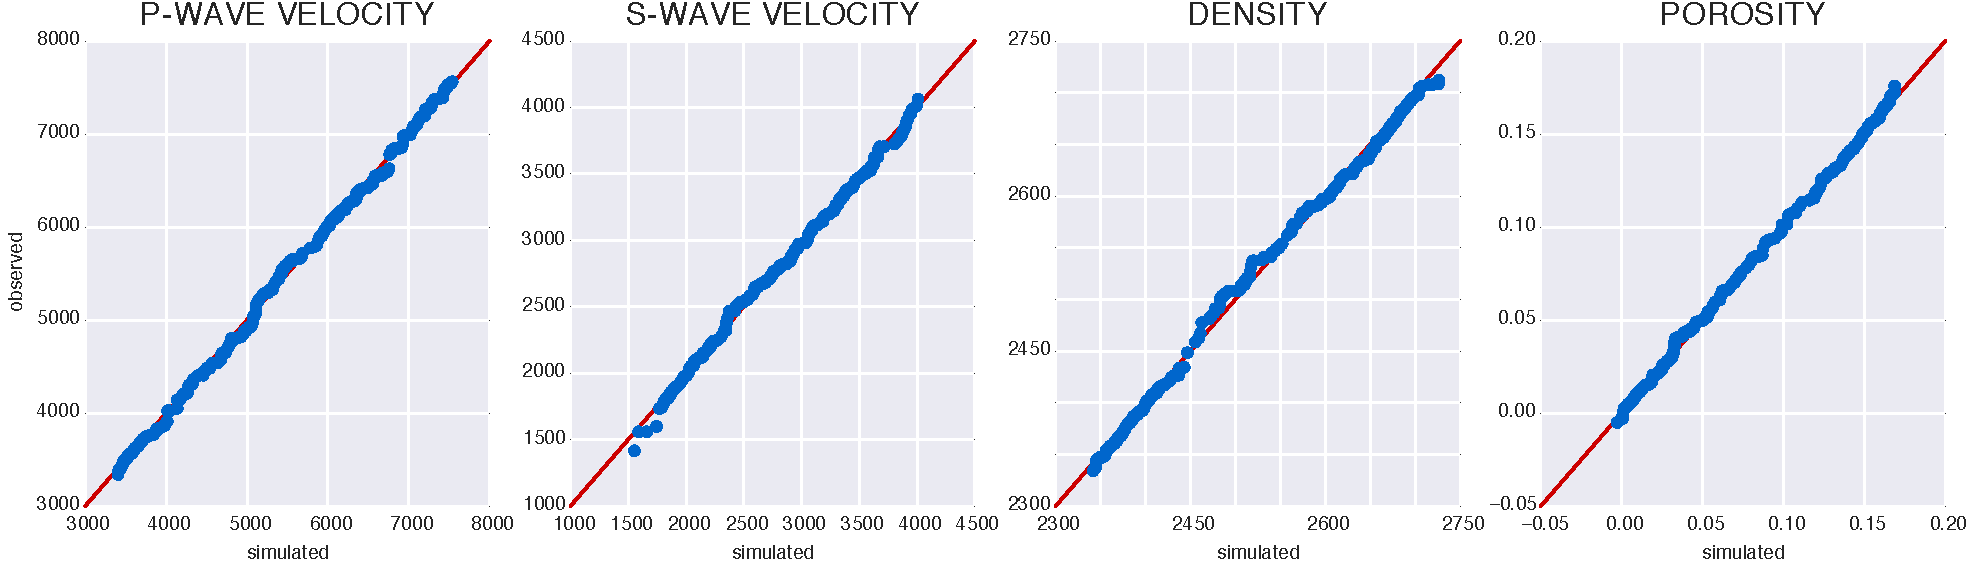
\includegraphics[width=1\textwidth]{fig/qqplot.pdf}
\caption{Q-Q plot of observed data versus inversion results data for $V_p$,
$V_s$, $\rho$ and $\phi$.}
\label{fig:qqplot}.
\end{figure}
Recently a measure of structural similarity (SSIM) that compares local patterns
between two images has been developed by \citet{Wang2004}. The SSIM index is a
decimal value between \SIlist{0;1}{}, where value 1 is only reachable in the
case of two identical sets of data. \Cref{fig:SSIM} shows the SSIM between the
reference model and one random SGS realization and between the reference model
and the inversion result for $P$-wave and $S$-wave velocity, density and
porosity.
\begin{figure}[!ht]
        \centering
        \begin{subfigure}[b]{.35\textwidth}
                \caption{SGS random realization}
                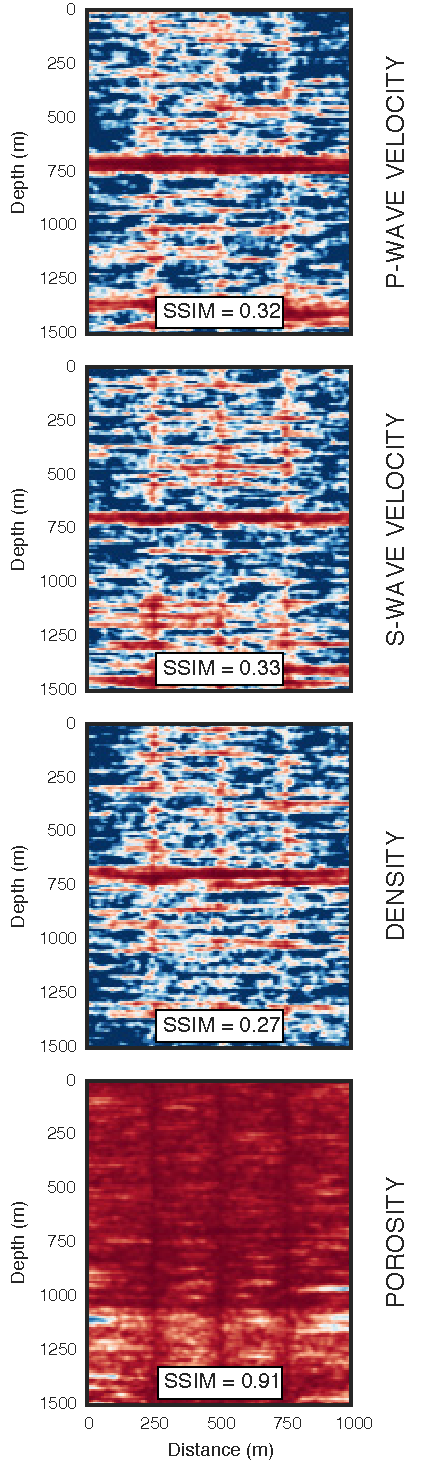
\includegraphics[width=\textwidth]{fig/ssim_a.pdf}
                \label{fig:ssim_a}
        \end{subfigure}%
        \begin{subfigure}[b]{.35\textwidth}
                \caption{Final inversion results}
                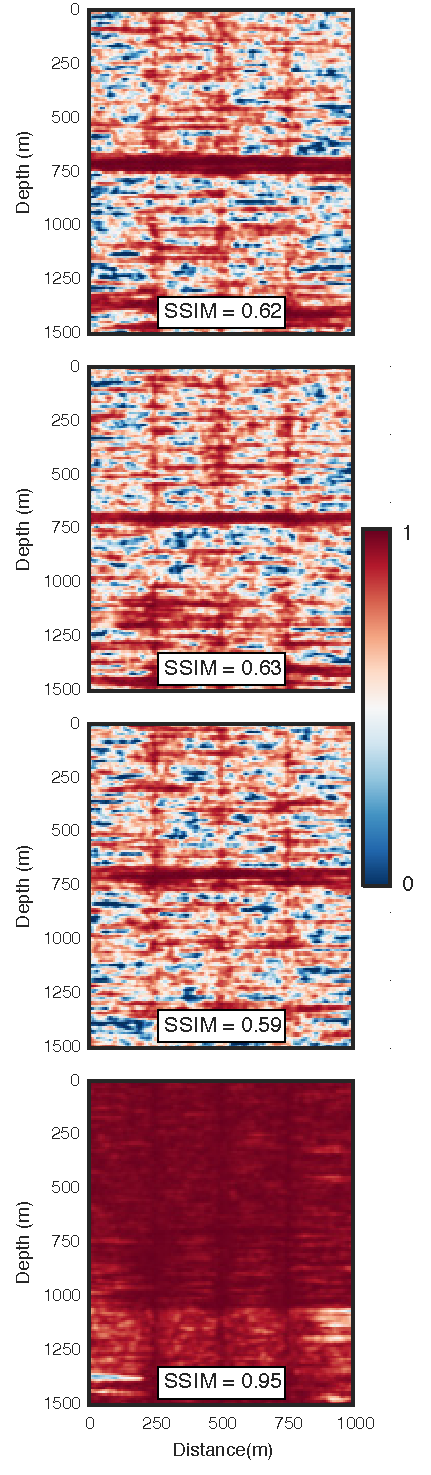
\includegraphics[width=\textwidth]{fig/ssim_b.pdf}
                \label{fig:ssim_b}
        \end{subfigure}
        \caption{Structural similarity index (SSIM) between the reference model
and one random SGS realization and between the reference model and the inversion
result for $V_p$, $V_s$, $\rho$ and $\phi$.}
        \label{fig:SSIM}
\end{figure}
The inversion results shows a SSIM index of about \num{0.6} for $V_p$, $V_s$ and
$\rho$. Compared to the random SGS realizations set, the inversion results are
significantly improved in terms of similarity with the reference models. The
$\phi$ field shows a SSIM index close to \num{1} for both SGS realization and
inversion results. This is quite normal as the $\phi$ distribution shows a low
variance for each layers (refer to \cref{tab:well-log}). If we focus at the
reservoir level (\SIrange{1050}{1300}{\metre}) we observe a clear improvement of
the similarity for the inversion results (SSIM=\num{0.89}) over the SGS
realization result (SSIM=\num{0.82}) as shown in \cref{fig:SSIM_res}. Indeed, as
we perform the \ce{CO2} flow simulation within this unit, we increase the number
of data in the optimization (i.e.\ the optimization is done for both static and
dynamic data), resulting in an increased similarity at the reservoir level
compared to the rest of the model.
\begin{figure}[!ht]
        \centering
        \begin{subfigure}[b]{.5\textwidth}
                \caption{SGS random realization}
                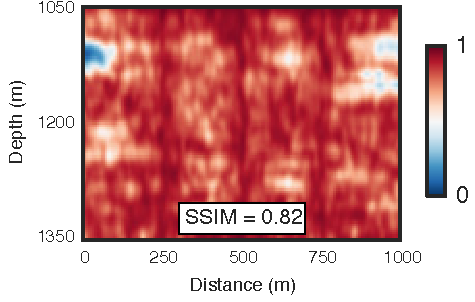
\includegraphics[width=\textwidth]{fig/ssim_res_a.pdf}
                \label{fig:ssim_res_a}
        \end{subfigure}%
        \begin{subfigure}[b]{.5\textwidth}
                \caption{Final inversion results}
                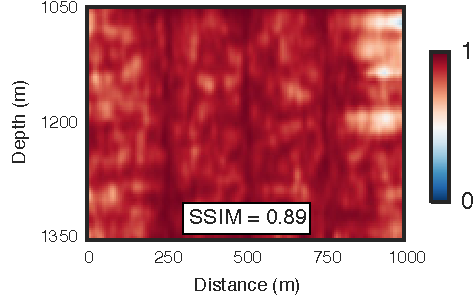
\includegraphics[width=\textwidth]{fig/ssim_res_b.pdf}
                \label{fig:ssim_res_b}
        \end{subfigure}
        \caption{Structural similarity index (SSIM) between the reference model
and one random SGS realization and between the reference model and the inversion
result for porosity field at the reservoir level.}
        \label{fig:SSIM_res}
\end{figure}
\section{Conclusion}
In our approach, we used the gradual deformation parametrization to obtain our
models for both static and dynamic data, however the probability perturbation
method \citep{Caers2006} could also be applied. This method explicitly deals
with the inverse problem of combining prior probabilities with pre-posterior
probabilities derived from the data.\\
 As the time lapse seismic differences due to the \ce{CO2} injection can be
relatively weak or spatially isolated, we argue that it is important to perform
full-wave forward modeling to capture most of the physics in the modeled seismic
data. However, this step can be very computationally demanding. In this work, we
used a Graphical Processing Unit (GPU) accelerated version of the viscoelastic
finite-difference time-domain forward modeling of \citep{Bohlen2002} developed
by \citep{Gab2014}, which allowed us reducing the run-time by more than 2 orders
of magnitude over the original parallel CPU version on a standard workstation.\\
% \section{Conclusion}
The objective of this study was to develop an inversion workflow to obtain
reservoir properties such as $V_p$, $V_s$, $\rho$ and $\phi$ that are
sufficiently detailed and accurate to allow for reliable prediction of \ce{CO2}
distributions. To this end, we developed a two-step optimization procedure based
on gradual deformation parametrization of both static and dynamic data.
Numerical experiments based on a realistic heterogeneous saline aquifer model
indicates that, given initial static data, the inversion approach should allow
for faithful properties estimation and reliable prediction of the spatial
distribution of \ce{CO2}. Critical future work will need to explore the
application of this methodology to field data, as well as its extension to 3-D
scenarios.
\section{Acknowledgments}
The authors would like to acknowledge G. Fabien-Ouellet for providing the
GPU-accelerated viscoelastic finite-difference time-domain code. Financial
support was provided by a research grant from the Québec Ministry of Sustainable
Development, Environment, Fauna and Parks and the Canada Research Chair in
Assimilation of Geological and Geophysical Data for Stochastic Geological
Modeling.
